% !TEX TS-program = lualatex
\documentclass[10pt,a4paper]{article}

\usepackage{fontspec}
\usepackage[english]{babel}
\usepackage[a4paper,margin=18mm,columnsep=6mm]{geometry}
\usepackage{amsmath}
\usepackage{amssymb}
\usepackage{booktabs}
\usepackage{graphicx}
\usepackage{caption}
\usepackage{subcaption}
\usepackage{float}
\usepackage{microtype}
\usepackage{placeins}
\usepackage[hidelinks]{hyperref}

\setmainfont{NewCM10-Regular.otf}[
  BoldFont=NewCM10-Bold.otf,
  ItalicFont=NewCM10-Italic.otf,
  BoldItalicFont=NewCM10-BoldItalic.otf
]
\setsansfont{NewCMSans10-Regular.otf}[
  BoldFont=NewCMSans10-Bold.otf,
  ItalicFont=NewCMSans10-Oblique.otf,
  BoldItalicFont=NewCMSans10-BoldOblique.otf
]
\setmonofont{NewCMMono10-Regular.otf}[
  BoldFont=NewCMMono10-Bold.otf,
  ItalicFont=NewCMMono10-Italic.otf,
  BoldItalicFont=NewCMMono10-BoldOblique.otf,
  Scale=0.9
]

\graphicspath{{assets/report/}}
\captionsetup{font=small,labelfont=bf}
\captionsetup[subfigure]{font=footnotesize}
\setlength{\parindent}{0.9em}
\setlength{\parskip}{0pt}
\setlength{\tabcolsep}{4pt}
\emergencystretch=1.5em
\raggedbottom

\newcommand{\mse}{\operatorname{MSE}}
\newcommand{\rmse}{\operatorname{RMSE}}

\title{\vspace{-1.2em}\bfseries Conditional Reconstruction of Sea-Ice Fields from Sparse Satellite Tracks}
\author{\small Experimental report}
\date{\vspace{-1.0em}}

\begin{document}
\maketitle

\begin{abstract}
We study conditional reconstruction of sea-ice fields from sparse satellite observations. Each observation is a set of narrow tracks: a binary mask specifies where the satellite passed over the domain, and the measured values on that mask are used as conditioning information. The report compares two conditioning strategies for diffusion/flow-matching models: inference-time gradient guidance and explicit input concatenation. The evaluation is deliberately broader than track-wise mean squared error, because a useful data-assimilation model should also reproduce the distribution of plausible fields away from the observed tracks.
\end{abstract}

\section{Problem Setting}

The target field is defined on a $320\times256$ grid with two physical channels: sea-ice concentration and sea-ice thickness. The conditioning observation is written as $(m,y)$, where $m$ is a binary satellite-track mask and $y=m\odot x$ contains the true field values only at observed pixels. The mask covers a small fraction of the domain, so the inverse problem is intrinsically underdetermined: many physically reasonable ice fields can agree with the same tracks.

This makes a purely pointwise evaluation incomplete. A track-restricted $\mse$ measures whether the reconstruction respects the known pixels, but it does not tell whether the unobserved part has realistic spatial structure, tails, marginal statistics, or uncertainty. The more relevant object is the conditional distribution $p(x\mid m,y)$: the model should place mass on fields that both match the tracks and remain statistically consistent with the training climatology.

\section{Conditioning Strategies}

\paragraph{Gradient guidance.}
The gradient-based method keeps the denoiser unconditional. During sampling, the current estimate of the final field is compared with the observed values on the mask, and the gradient of this discrepancy is added to the velocity update. In effect, the prior model is corrected at inference time by a data-consistency term. This is flexible because no conditional retraining is required, but it can be sensitive to the guidance scale and to the mismatch between the correction and the learned flow.

\paragraph{Concatenation conditioning.}
The concatenation method makes the condition part of the neural input. At every denoising step the U-Net receives the noisy field, coordinate channels, the track mask, and the observed values on the tracks. The model therefore learns during training how satellite-track geometry should constrain the reconstruction. This approach is less modular than gradient guidance, but the conditioning signal is aligned with the learned dynamics of the sampler.

\section{Controlled Lorenz-63 Experiment}

Lorenz-63 is used as a compact diagnostic problem where the geometry of the target distribution is visible. The system is generated with $\sigma=10$, $\rho=28$, $\beta=8/3$ and split into 200000 training states, 20000 validation states, and 20000 test states. Sparse observations are simulated by revealing either random coordinates or a fixed coordinate of the three-dimensional state.

\begin{table}[H]
\centering
\footnotesize
\begin{tabular}{llcccc}
\toprule
Method & Conditioning protocol & Full $\rmse$ & Obs. $\rmse$ & Unobs. $\rmse$ & Posterior $W_1$ \\
\midrule
Mean-fill baseline & random 1--2 coordinates & 5.926 & 0.000 & 8.387 & -- \\
Gradient guidance & random 1--2 coordinates & 11.900 & 11.912 & 11.887 & 15.018 \\
Mean-fill baseline & fixed $y$ coordinate & 5.926 & 0.000 & 8.387 & -- \\
Concat conditioning & fixed $y$ coordinate & 5.621 & 0.208 & 7.953 & 2.094 \\
\bottomrule
\end{tabular}
\caption{Lorenz-63 summary. The first two rows and the last two rows use different conditioning protocols, so the table should be read as a diagnostic of each conditioning mechanism rather than as a single leaderboard.}
\label{tab:lorenz}
\end{table}

The concatenation model gives a much tighter posterior in the fixed-coordinate setting: the Wasserstein distance drops to $2.094$, and the observed coordinate is held nearly exactly. The gradient-guided sampler is less stable in this small test. Its correction can satisfy neither the attractor geometry nor the observation particularly well when the guidance term is not balanced with the learned prior.

\begin{figure}[H]
\centering
\begin{subfigure}{0.49\textwidth}
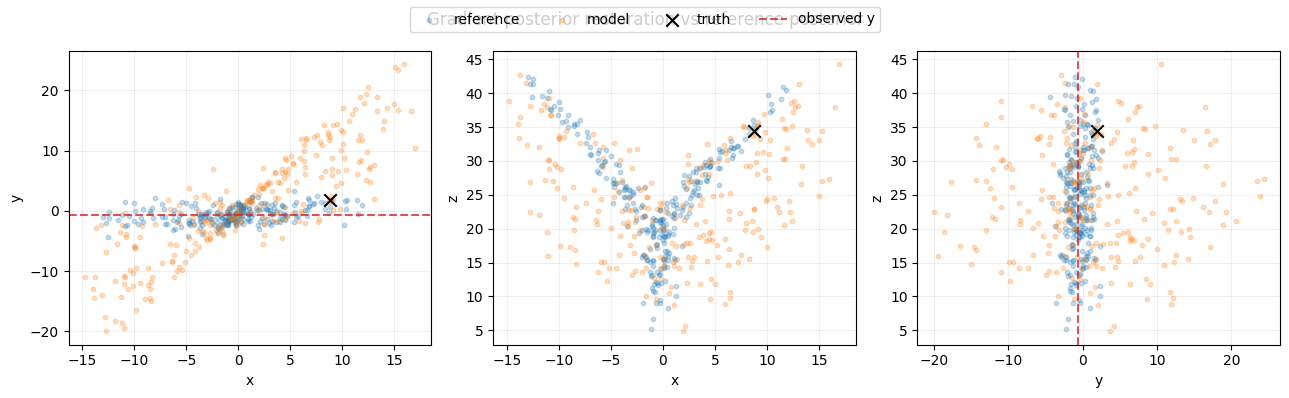
\includegraphics[width=\linewidth]{lorenz-gradient-posterior.png}
\caption{One test state. Conditioning: an observed $y$ coordinate with observation noise $\sigma_{\mathrm{obs}}=0.15$.}
\end{subfigure}
\hfill
\begin{subfigure}{0.49\textwidth}
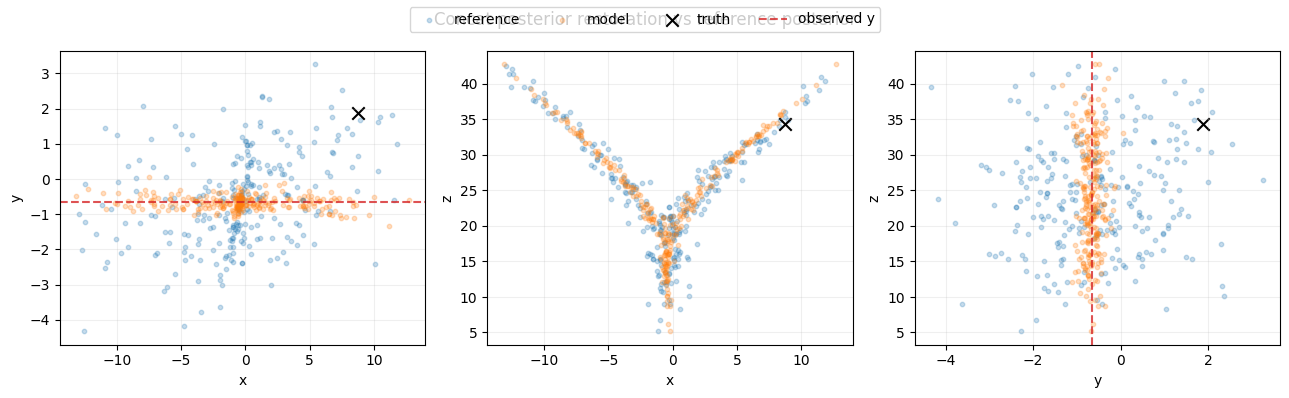
\includegraphics[width=\linewidth]{lorenz-concat-posterior.png}
\caption{One test state. Conditioning: the exact $y$ coordinate, with mask $(0,1,0)$.}
\end{subfigure}
\caption{Conditional posterior samples for Lorenz-63. Blue points denote the reference posterior, orange points denote model samples, the black marker is the true state, and the red dashed line shows the observed coordinate.}
\label{fig:lorenz-posterior}
\end{figure}

\section{Sea-Ice Reconstruction}

The sea-ice experiments use the two-channel $320\times256$ fields described above. In the single-sample reconstructions, a real satellite swath is used as the conditioning mask. The observed values are the true concentration and thickness on that mask and zero elsewhere. Track-wise errors are reported after denormalization and are computed only on observed pixels.

\begin{figure}[H]
\centering
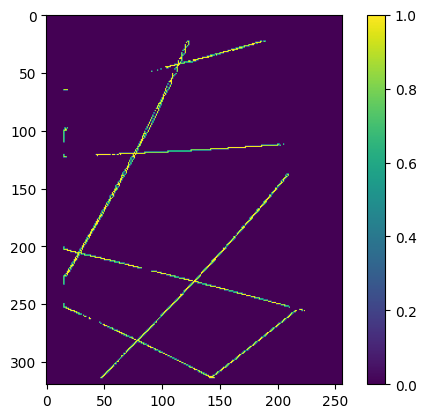
\includegraphics[width=0.55\linewidth]{ice-real-swath-mask.png}
\caption{Real satellite swath used as conditioning in the single-sample reconstruction experiments. The visible pixels define where concentration and thickness are observed; all other pixels must be inferred from the learned prior.}
\label{fig:swath-mask}
\end{figure}

\begin{table}[H]
\centering
\small
\begin{tabular}{lcc}
\toprule
Method & Concentration track $\mse$ & Thickness track $\mse$ \\
\midrule
Gradient guidance & 0.02765 & 0.12282 \\
Concat conditioning & 0.00041 & 0.00160 \\
\bottomrule
\end{tabular}
\caption{Mean track-restricted $\mse$ after denormalization. The examples are validation fields conditioned on the same real swath mask; the metric measures agreement with the observed tracks, not the full-field distribution.}
\label{tab:ice-mse}
\end{table}

\subsection{Gradient Guidance}

For the gradient-guided experiment, 18 validation fields are reconstructed under the same real swath condition. Sampling uses 50 denoising steps and a guidance scale of 50. The method produces coherent ice shapes, but it does not enforce the observations as tightly as the conditional model, especially for thickness.

\begin{figure}[H]
\centering
\begin{subfigure}{0.49\textwidth}
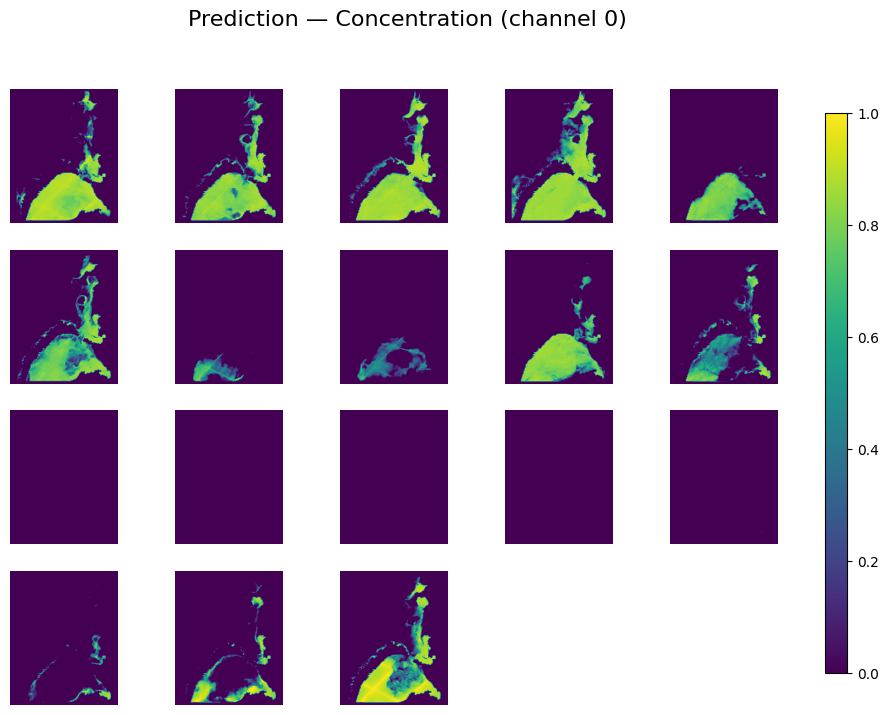
\includegraphics[width=\linewidth]{ice-gradient-prediction.png}
\caption{Predictions for 18 validation examples. Conditioning: one real swath mask and the observed concentration/thickness values on that mask.}
\end{subfigure}
\hfill
\begin{subfigure}{0.49\textwidth}
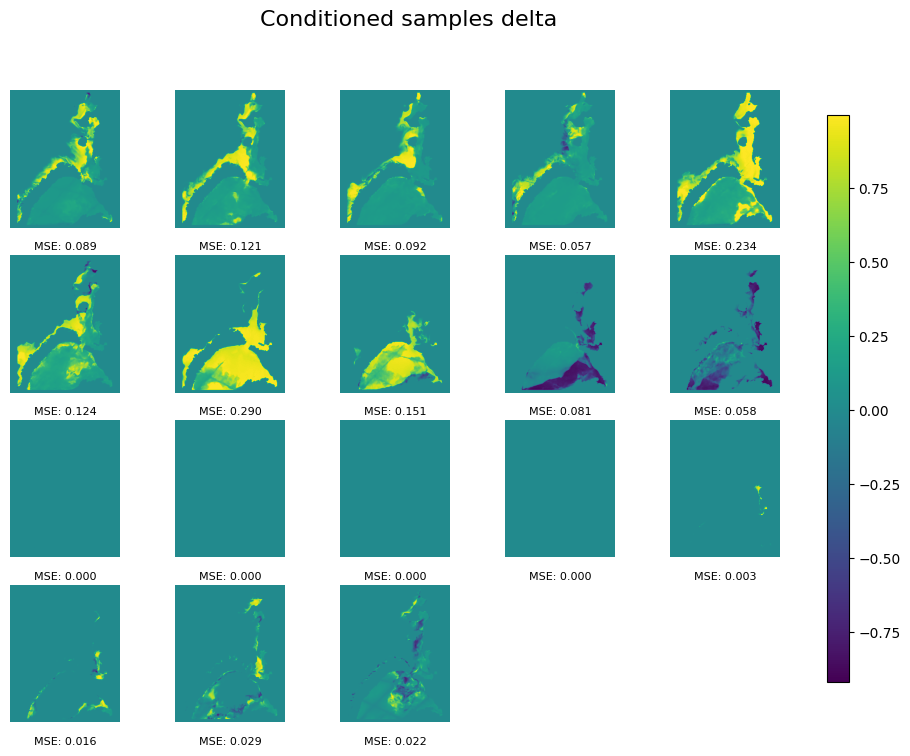
\includegraphics[width=\linewidth]{ice-gradient-residual.png}
\caption{Residuals for the same examples and conditioning. Errors appear near ice edges and inside several large ice-covered regions.}
\end{subfigure}
\caption{Gradient-guided reconstruction of sea-ice concentration. The method adapts an unconditional prior at inference time, but the track error remains relatively high: $2.765\cdot10^{-2}$ for concentration and $1.2282\cdot10^{-1}$ for thickness.}
\label{fig:gradient-ice}
\end{figure}

\subsection{Concatenation Conditioning}

The concatenation experiment reconstructs 25 validation fields with the same real swath mask and the corresponding observed values on the tracks. Sampling again uses 50 denoising steps. Because the model sees the mask and observations throughout training and sampling, it follows the conditioning much more closely.

\begin{figure}[H]
\centering
\begin{subfigure}{0.49\textwidth}
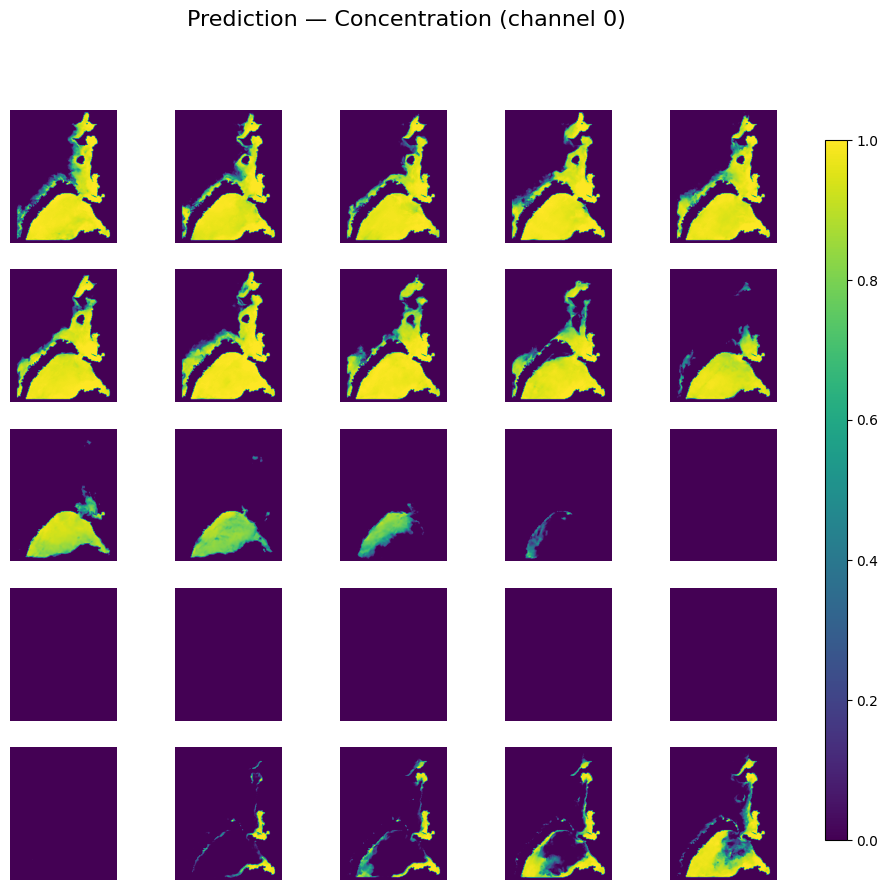
\includegraphics[width=\linewidth]{ice-concat-prediction.png}
\caption{Predictions for 25 validation examples. Conditioning: the real swath mask and the observed concentration/thickness values on that mask.}
\end{subfigure}
\hfill
\begin{subfigure}{0.49\textwidth}
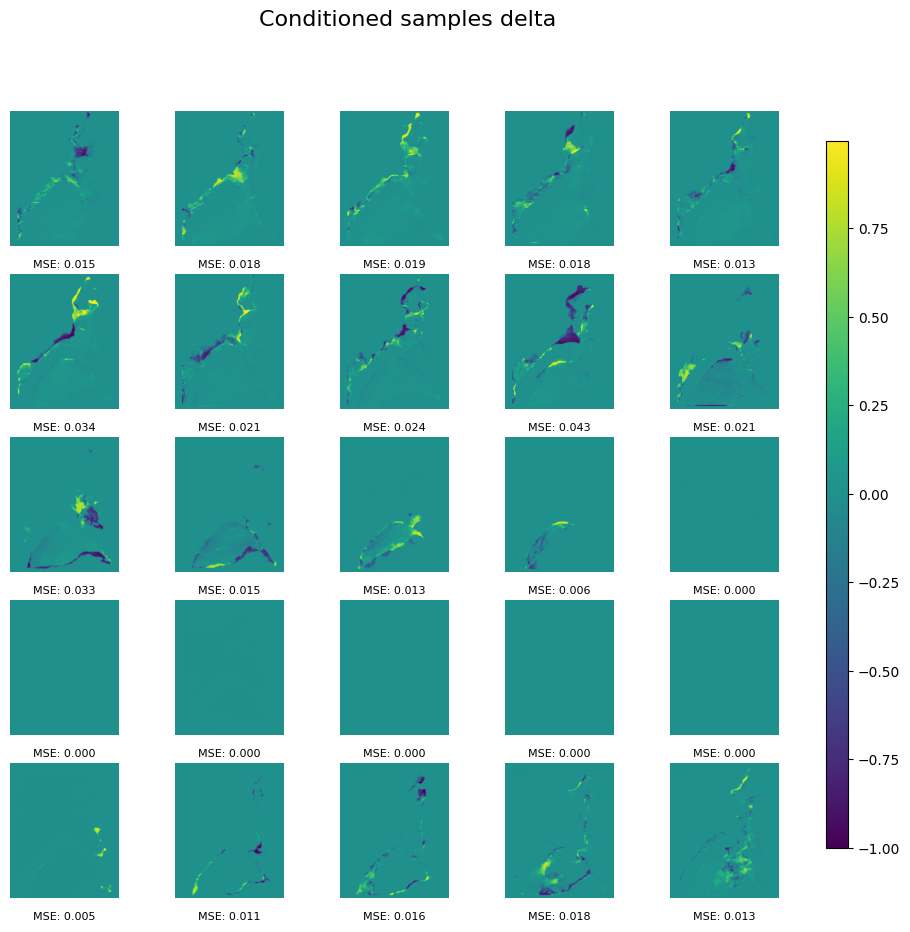
\includegraphics[width=\linewidth]{ice-concat-residual.png}
\caption{Residuals for the same examples and conditioning. The remaining error is concentrated around boundaries and thin structures.}
\end{subfigure}
\caption{Concatenation-based reconstruction of sea-ice concentration. Track consistency is substantially stronger than with gradient guidance: $4.1\cdot10^{-4}$ for concentration and $1.60\cdot10^{-3}$ for thickness.}
\label{fig:concat-ice}
\end{figure}

\section{Ensemble Evaluation}

Single reconstructions hide the uncertainty of the inverse problem. To probe the conditional distribution, an ensemble is generated for 48 validation cases. Each case is conditioned on a synthetic 15-track mask and on the true field values along those tracks. The mask covers approximately $3.85\%$ of the grid. For each condition, 10 samples are drawn with 10 denoising steps using a DOPRI5 solver.

\begin{table}[H]
\centering
\small
\begin{tabular}{lc}
\toprule
Metric & Value \\
\midrule
RMSE of ensemble mean & $0.253\pm0.188$ \\
Masked RMSE & $0.109\pm0.087$ \\
RMSE of individual member & $0.303\pm0.209$ \\
Mean ensemble spread & $0.077\pm0.173$ \\
\bottomrule
\end{tabular}
\caption{Ensemble summary over 48 validation cases. Conditioning: a synthetic 15-track mask per case and observed concentration/thickness values on the tracks. Averaging the ensemble improves RMSE relative to a typical individual member, while the spread remains spatially uneven.}
\label{tab:ensemble}
\end{table}

\begin{figure}[H]
\centering
\begin{subfigure}{0.49\textwidth}
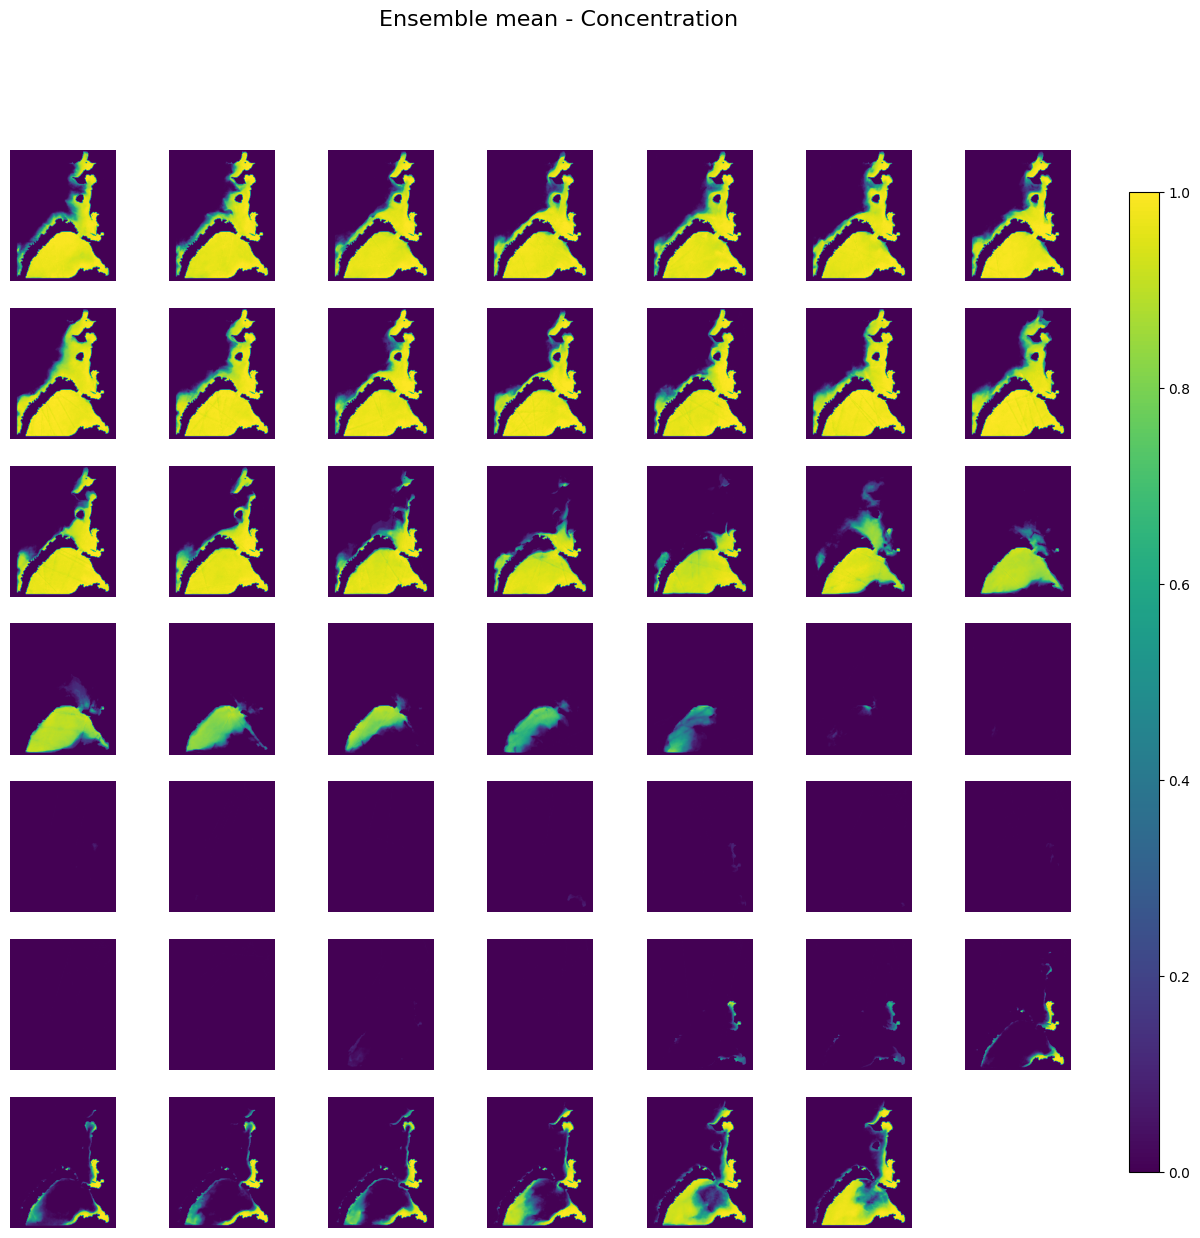
\includegraphics[width=\linewidth]{ice-ensemble-mean.png}
\caption{Ensemble mean for 48 validation examples. Conditioning: synthetic 15-track masks and observed values on those tracks.}
\end{subfigure}
\hfill
\begin{subfigure}{0.49\textwidth}
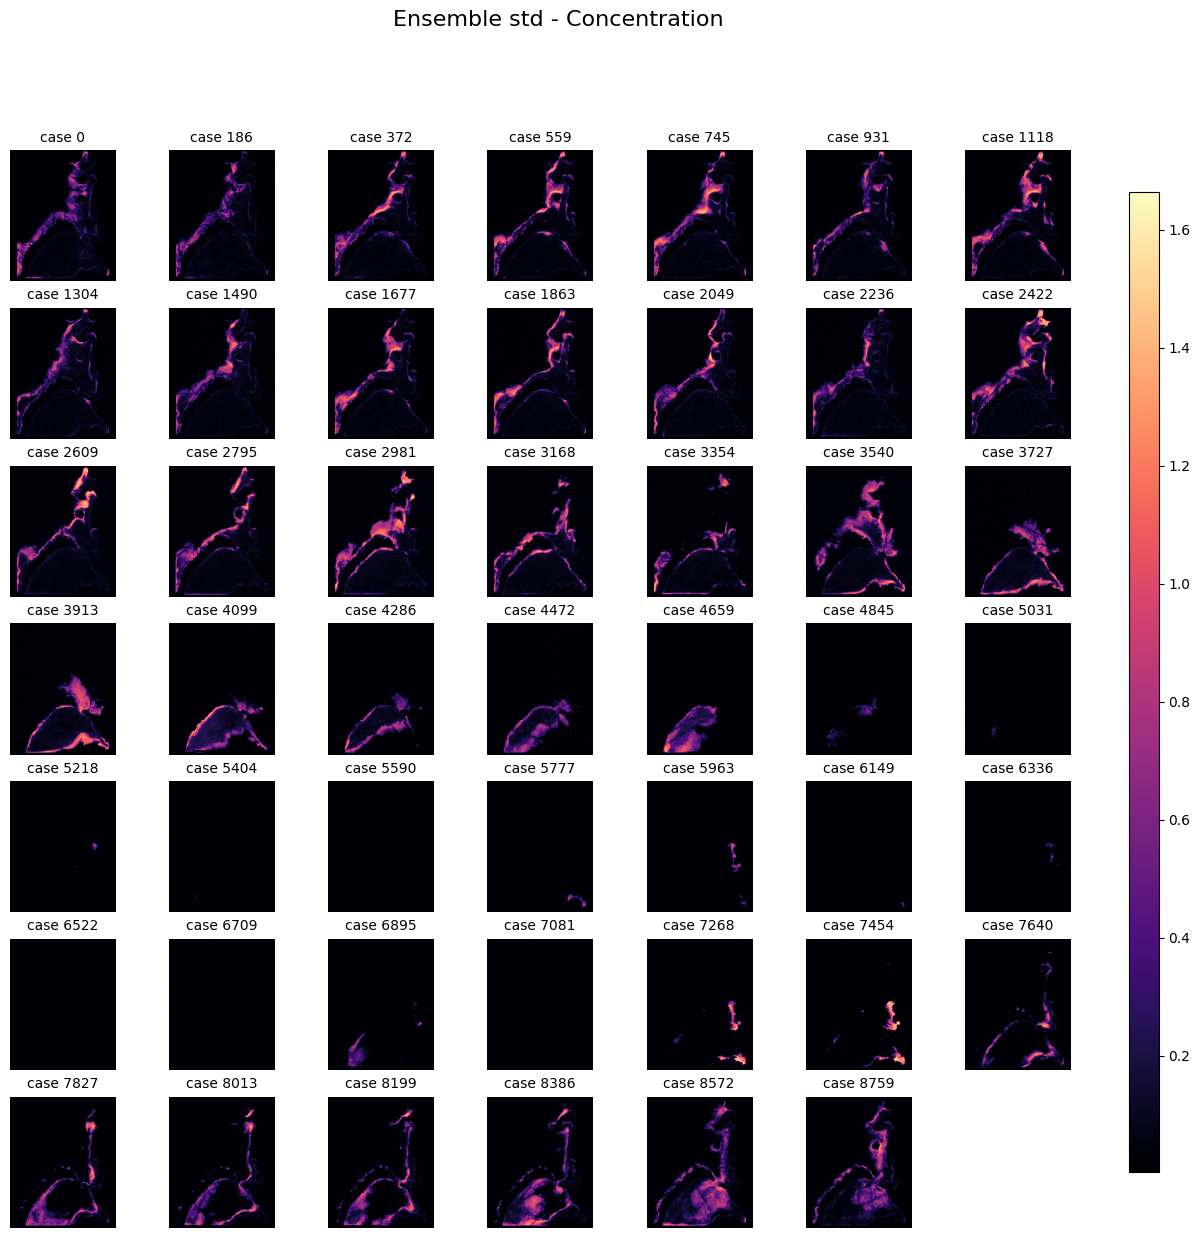
\includegraphics[width=\linewidth]{ice-ensemble-spread.png}
\caption{Ensemble standard deviation for the same examples and conditioning. The largest spread occurs near ice boundaries and weakly constrained regions.}
\end{subfigure}
\caption{Ensemble reconstruction of sea-ice concentration. The mean summarizes the central conditional estimate, while the spread indicates where multiple plausible completions remain.}
\label{fig:ensemble}
\end{figure}

\begin{figure}[H]
\centering
\begin{subfigure}{\textwidth}
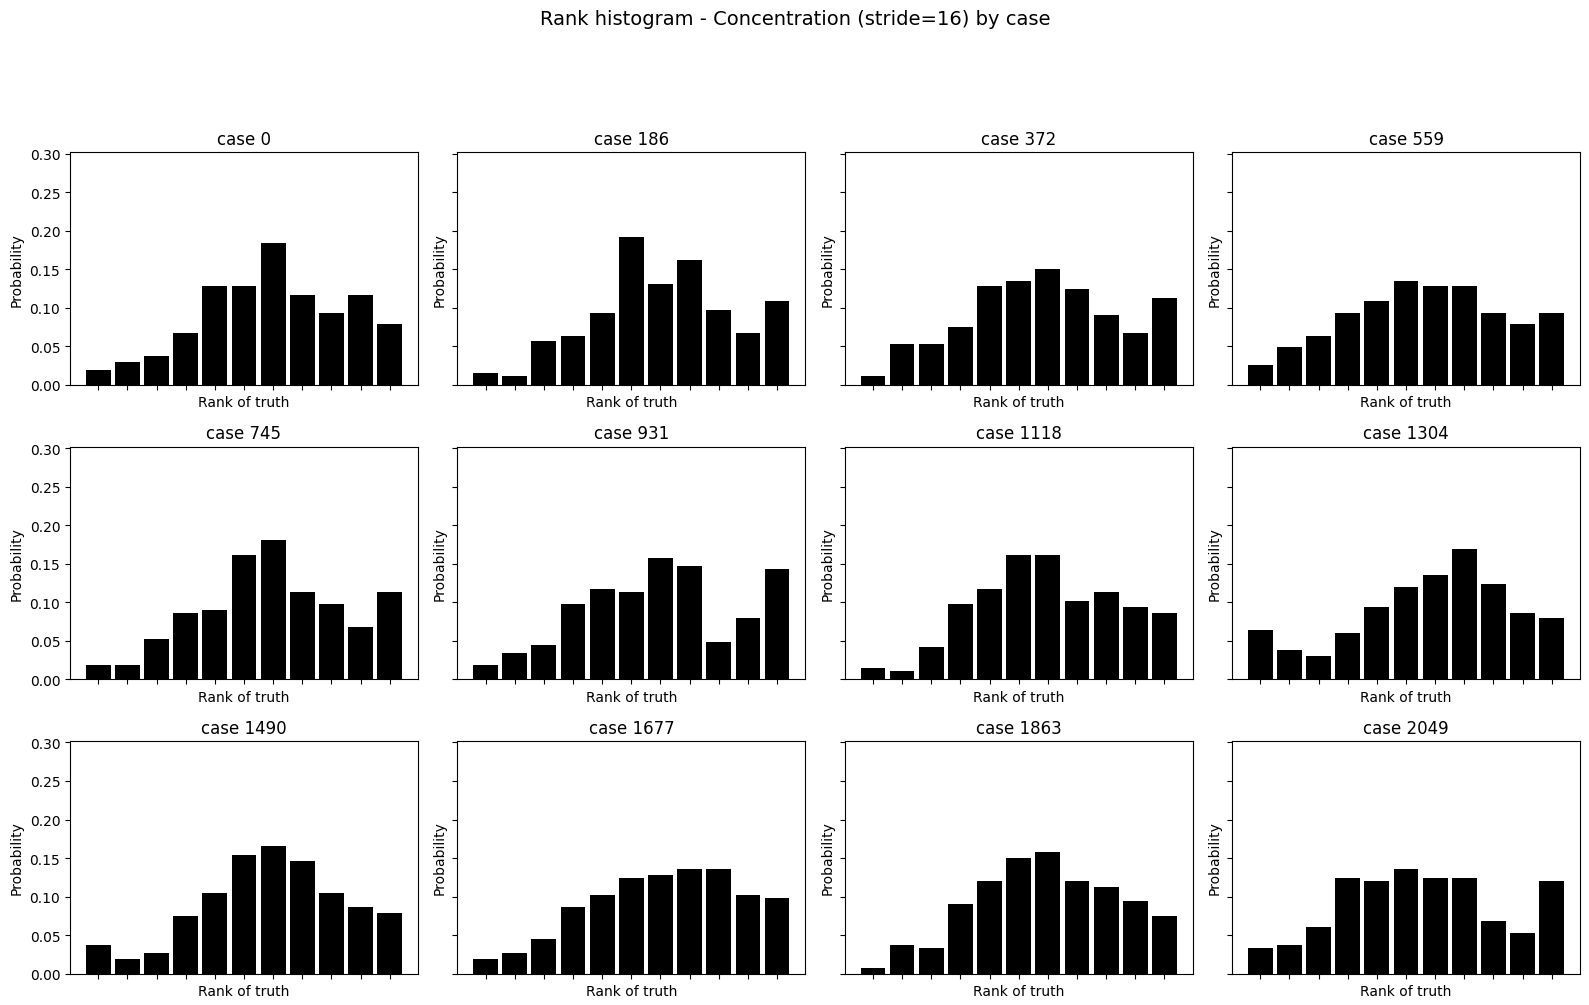
\includegraphics[width=\linewidth]{rank_cases/rank_cases_01.png}
\caption{Rows 1--3. Each small panel is a separate validation case.}
\end{subfigure}
\vspace{0.4em}
\begin{subfigure}{\textwidth}
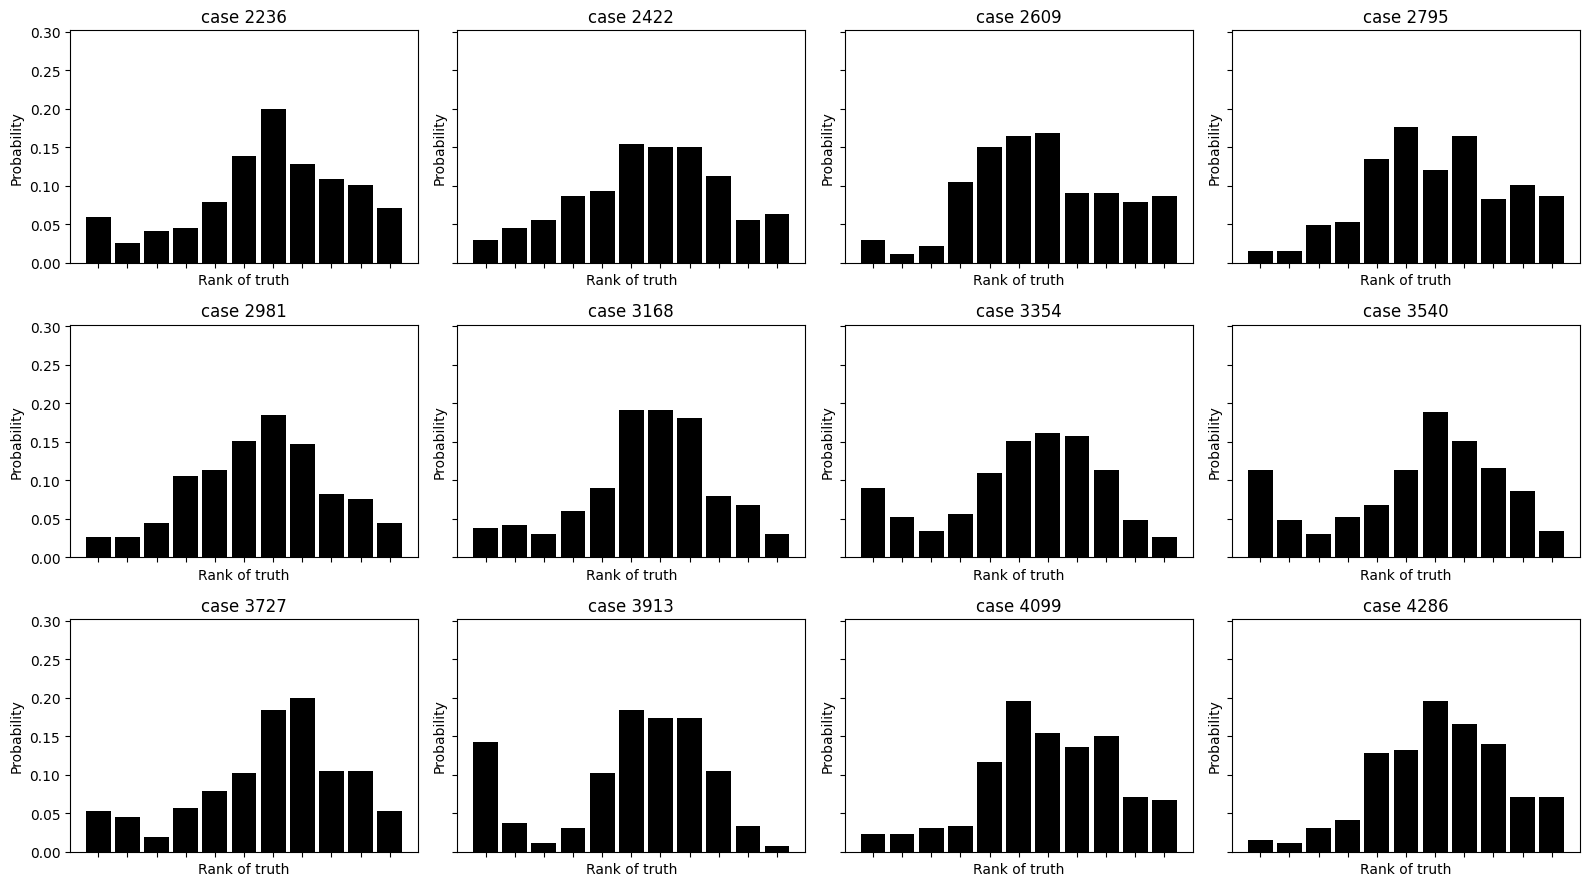
\includegraphics[width=\linewidth]{rank_cases/rank_cases_02.png}
\caption{Rows 4--6. Each small panel is a separate validation case.}
\end{subfigure}
\caption{Per-case rank histograms for concentration. Examples: 48 validation cases; conditioning: one synthetic 15-track mask per case with observed concentration/thickness values on the tracks. Showing the histograms case by case is more informative than pooling them into a single curve, because calibration errors vary strongly across conditions.}
\label{fig:rank-hist-a}
\end{figure}

\begin{figure}[H]
\centering
\begin{subfigure}{\textwidth}
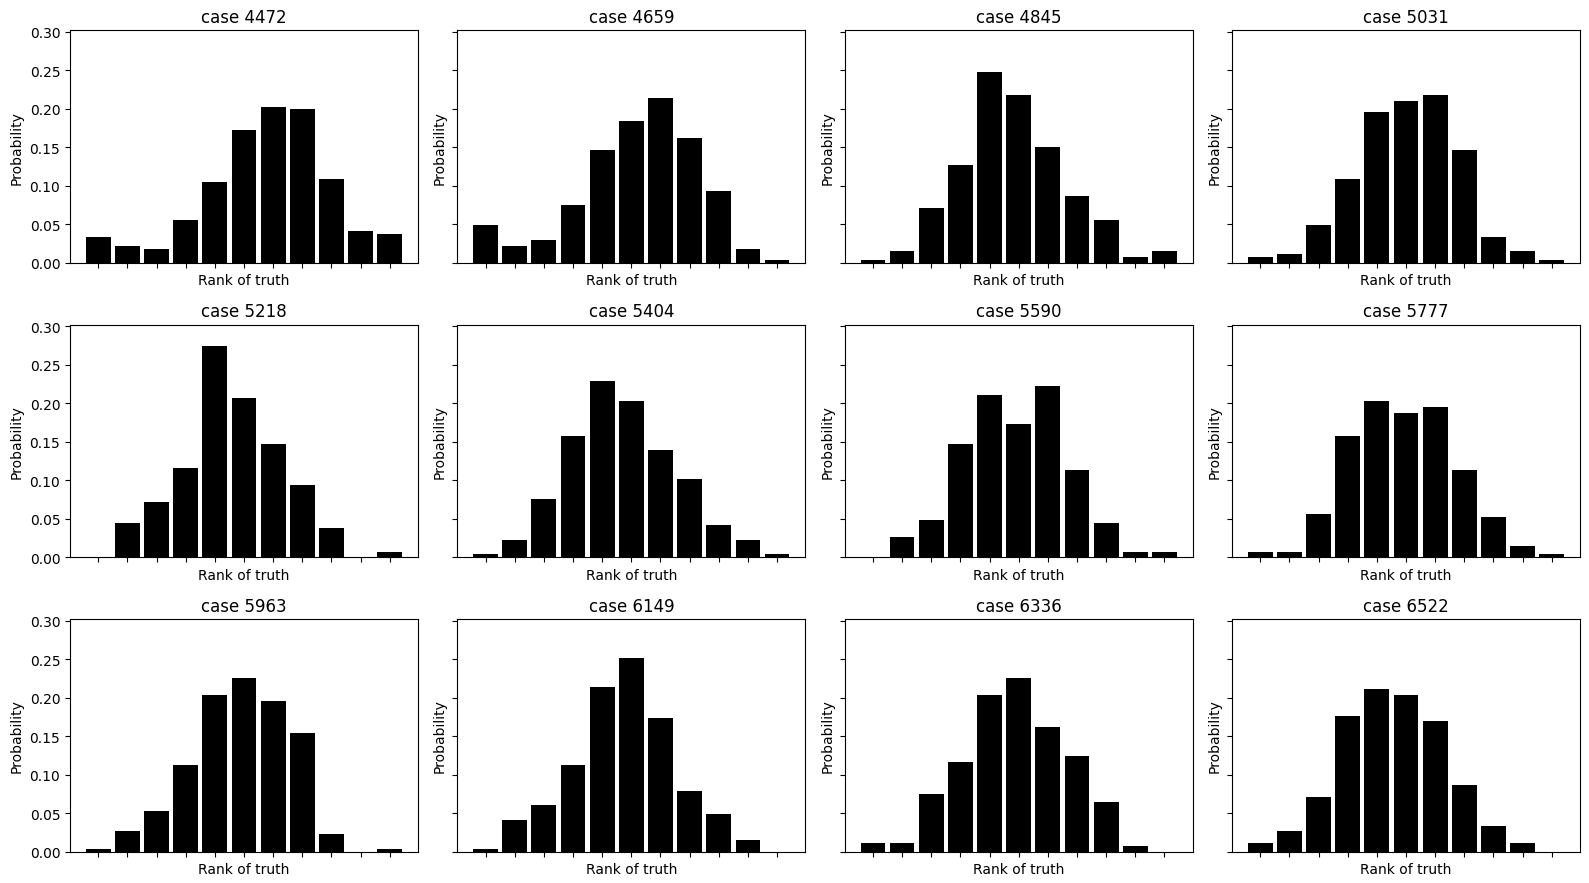
\includegraphics[width=\linewidth]{rank_cases/rank_cases_03.png}
\caption{Rows 7--9. Each small panel is a separate validation case.}
\end{subfigure}
\vspace{0.4em}
\begin{subfigure}{\textwidth}
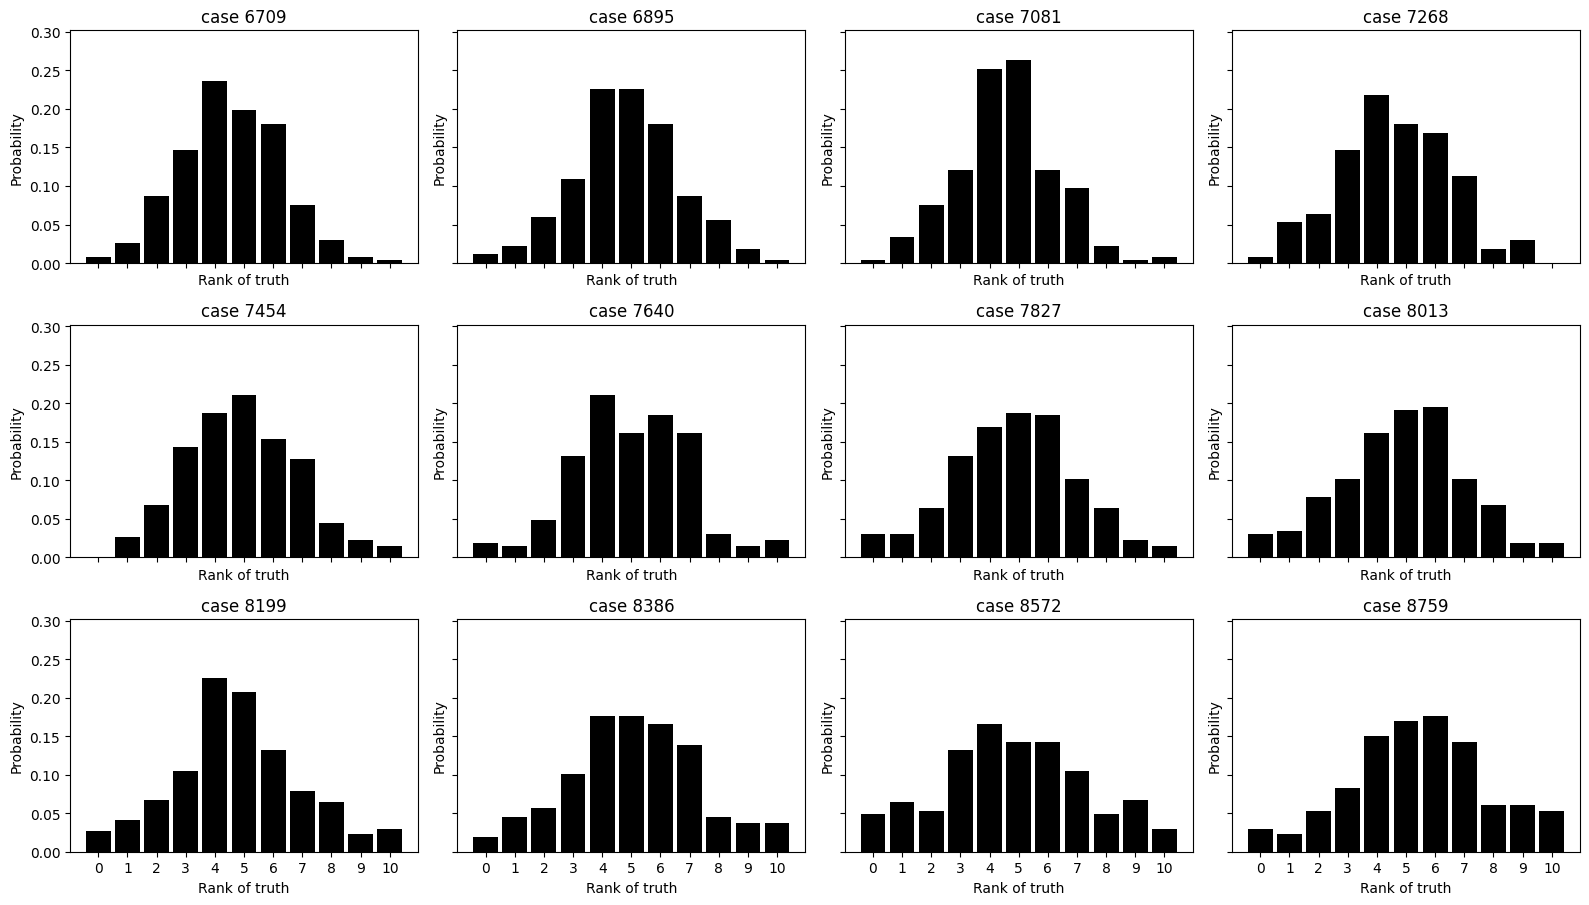
\includegraphics[width=\linewidth]{rank_cases/rank_cases_04.png}
\caption{Rows 10--12. Each small panel is a separate validation case.}
\end{subfigure}
\caption{Continuation of the per-case concentration rank histograms for the same 48 validation cases and the same synthetic-track conditioning. Several panels are close to centered, while others place too much mass toward low or high ranks, indicating that ensemble calibration is condition-dependent.}
\label{fig:rank-hist-b}
\end{figure}

\section{Distributional Evaluation}

The final check compares real training fields with an unconditional generated subset from the concatenation model. The real set contains 60816 training fields; the generated set contains 1000 samples drawn with an empty mask, so no satellite tracks are provided as conditioning. This evaluates the learned marginal prior rather than a particular assimilation case. All statistics are computed over valid ocean pixels; for the plotted pixel distributions, 200000 pixels are sampled per channel.

\begin{figure}[H]
\centering
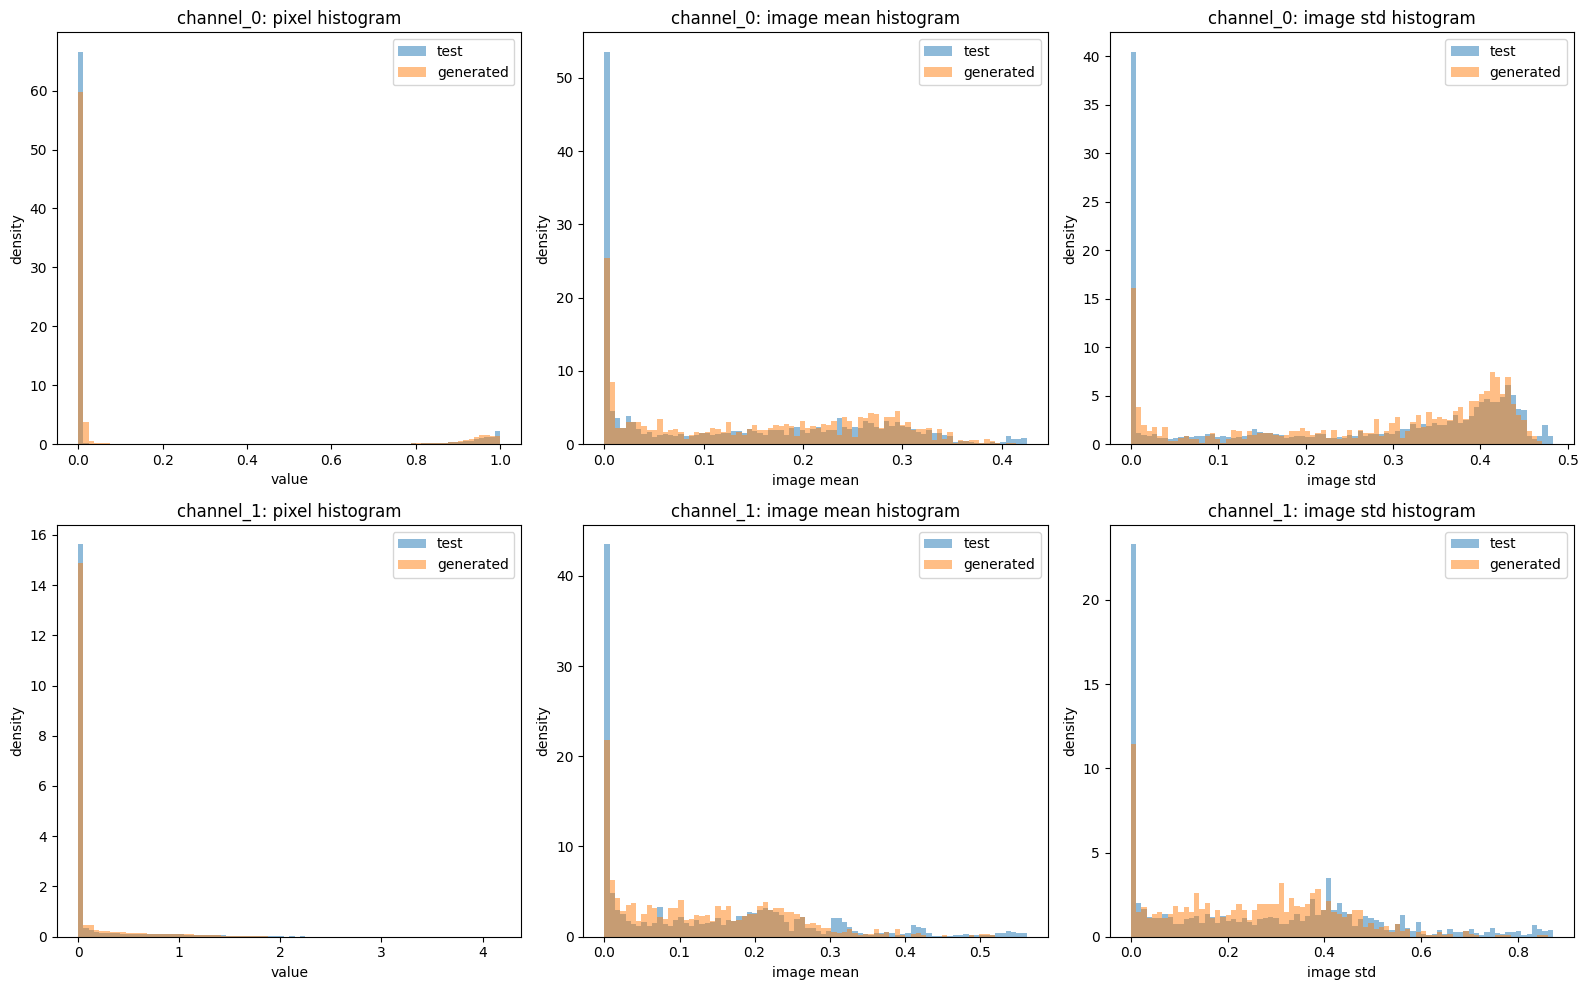
\includegraphics[width=\textwidth]{distribution-histograms.png}
\caption{Distributional histograms for concentration and thickness. Examples: 60816 real training fields versus 1000 generated fields. Conditioning for the generated set: empty mask, i.e. no observed satellite tracks. The panels compare pixel values, image means, and image standard deviations.}
\label{fig:distribution-hist}
\end{figure}

\begin{figure}[H]
\centering
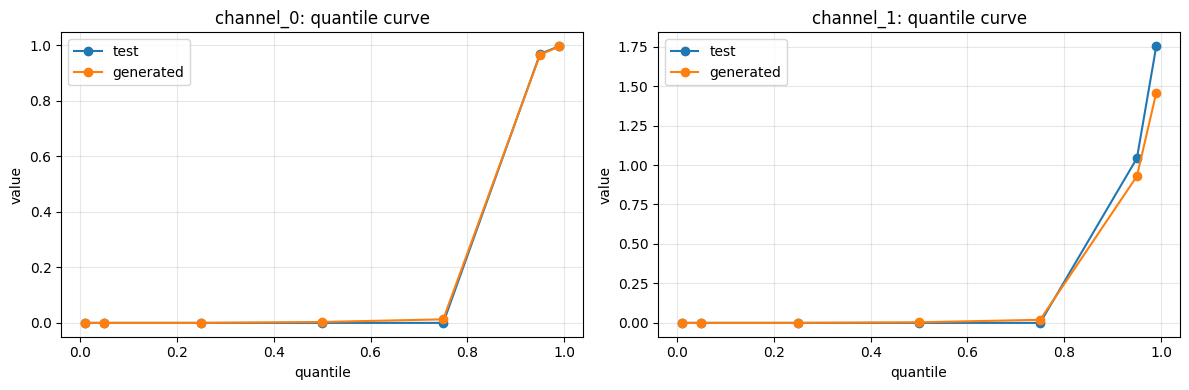
\includegraphics[width=0.78\textwidth]{distribution-quantiles.png}
\caption{Quantile comparison for the same real and generated examples. Conditioning for generated fields is absent, so the plot measures the marginal prior. Concentration is close in the upper quantiles, while thickness underrepresents the high tail: the generated 95\% and 99\% quantiles are 0.929 and 1.459, compared with 1.043 and 1.753 for real fields.}
\label{fig:distribution-quantiles}
\end{figure}

The pixel mean for generated concentration is higher than in the training set, $0.158$ versus $0.136$. Thickness has a closer mean, $0.131$ versus $0.135$, but the upper tail is visibly weaker in the generated samples. This is precisely the type of discrepancy that can be missed by track-wise $\mse$: the model may satisfy sparse observations while still producing a biased climatology in the unobserved part of the field.

\FloatBarrier

\section{Conclusion}

The experiments point to a clear baseline. Explicit concatenation conditioning is more reliable than inference-time gradient guidance for respecting sparse satellite tracks, both in the Lorenz diagnostic and in the sea-ice reconstructions. At the same time, track accuracy is only one part of the problem. A useful reconstruction model must also be evaluated as a conditional generator: its samples should match observed tracks, preserve realistic spatial variability, produce calibrated ensembles, and reproduce the marginal distribution of concentration and thickness, including the tails.

\end{document}
